\section*{Concurrent Counters (initial vs scalable/approximate)}
\begin{minipage}{.5\linewidth}
\begin{lstlisting}[language=c,xrightmargin=4pt]
typedef struct __counter_t {
  int value;
  pthread_mutex_t lock;
} counter_t;
void init(counter_t *c) {
  c->value = 0;
  Pthread_mutex_init(
          &c->lock, NULL);
}
int get(counter_t *c) {
  Pthread_mutex_lock(&c->lock);
  int rc = c->value;
  Pthread_mutex_unlock(&c->lock);
  return rc;
}
\end{lstlisting}
\end{minipage}
\begin{minipage}{.5\linewidth}
\begin{lstlisting}[language=c,xleftmargin=4pt,framextopmargin=2pt]
void increment(counter_t *c) {
  Pthread_mutex_lock(&c->lock);
  c->value++;
  Pthread_mutex_unlock(&c->lock);
}
void decrement(counter_t *c) {
  Pthread_mutex_lock(&c->lock);
  c->value--;
  Pthread_mutex_unlock(&c->lock);
}
\end{lstlisting}
  \begin{itemize}
  \item add locks to every read/write access to shared value
  \item thread-safe but too slow: scales poorly as \#threads grows
  \end{itemize}
\end{minipage}
\begin{lstlisting}[language=c]
typedef struct __counter_t {
    int global;                         // global count
    pthread_mutex_t glock;              // global lock
    int local[NUMCPUS];                 // per-CPU count
    pthread_mutex_t llock[NUMCPUS]; // ... and locks
    int threshold;                      // update freq
} counter_t;
// record threshold, init locks and vals of all local cnt/gloabl cnt
void init(counter_t *c, int threshold) {
    c->threshold = threshold;
    c->global = 0;
    pthread_mutex_init(&c->glock, NULL);
    int i;
    for (i = 0; i < NUMCPUS; i++) {
       c->local[i] = 0;
       pthread_mutex_init(&c->llock[i], NULL);
  }
}

// usually, just grab local lock and update local amount;
// once above `threshold', grab global lock, transfer local vals to it
void update(counter_t *c, int threadID, int amt) {
    int cpu = threadID % NUMCPUS;
    pthread_mutex_lock(&c->llock[cpu]);
    c->local[cpu] += amt;
    if (c->local[cpu] >= c->threshold) {
        // transfer to global (assumes amt > 0)
        pthread_mutex_lock(&c->glock);
        c->global += c->local[cpu];
        pthread_mutex_unlock(&c->glock);
        c->local[cpu] = 0;
    }
    pthread_mutex_unlock(&c->llock[cpu]);
}
\end{lstlisting}
\begin{minipage}{.48\linewidth}
\begin{lstlisting}[language=c]
int get(counter_t *c) {
  pthread_mutex_lock(&c->glock);
  int val = c->global;
  pthread_mutex_unlock(&c->glock);
  return val; // only approximate!
}
\end{lstlisting}
\end{minipage}
\begin{minipage}{.52\linewidth}
  \centering
  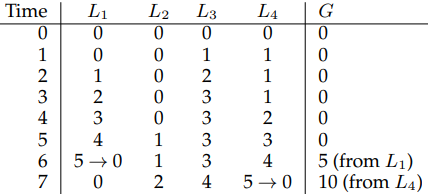
\includegraphics[width=.85\linewidth]{imgs/tracing_approx_cnter}
\end{minipage}
\begin{minipage}{.5\linewidth}
  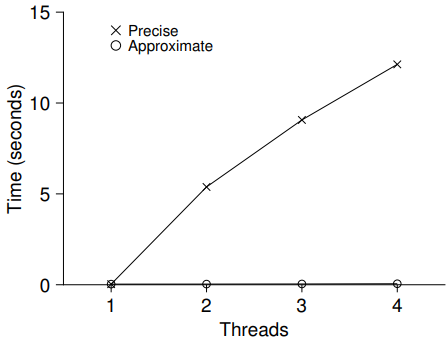
\includegraphics[width=.8\linewidth]{imgs/precise_approx_cnter}
\end{minipage}
\begin{minipage}{.5\linewidth}
  \centering
  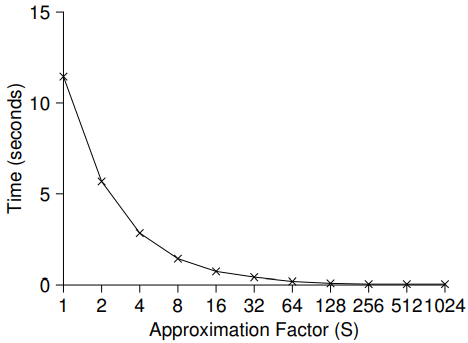
\includegraphics[width=.8\linewidth]{imgs/scaling_approx_cnter}
\end{minipage}
\section*{Concurrent Linked List (insertion and lookup)}
\begin{minipage}{.52\linewidth}
\begin{lstlisting}[language=c,xleftmargin=-4pt]
// basic node structure
typedef struct __node_t {
   int               key;
   struct __node_t   *next;
} node_t;
// basic list struct, used per list
typedef struct __list_t {
    node_t           *head;
    pthread_mutex_t  lock;
} list_t;
void List_Init(list_t *L) {
  L->head = NULL;
  pthread_mutex_init(&L->lock, NULL);
}
\end{lstlisting}
\end{minipage}
\begin{minipage}{.48\linewidth}
  \flushleft
  \begin{itemize}
  \item acquire lock upon entry to insert fn and release it upon exit
  \item if \texttt{malloc()} fails, the code must also release lock
  \item nearly 40\% bugs found on such rarely-taken code path
  \item \textbf{rearrange} code so that lock and release only surround actual critical section in insert code, $\because$ part of insert need no locking
  \item assume \texttt{malloc} itself thread-safe $\to$ no race conds and only updating shared list needs lock
  \end{itemize}
\end{minipage}
\begin{minipage}{.53\linewidth}
\begin{lstlisting}[language=c,xleftmargin=-4pt]
int List_Insert(list_t *L,int key)
{
  pthread_mutex_lock(&L->lock);
  node_t *new = malloc(sizeof node_t);
  if (new == NULL) {
    perror("malloc");
    pthread_mutex_unlock(&L->lock);
    return -1; // fail
  }
  new->key = key;
  new->next = L->head;
  L->head = new;
  pthread_mutex_unlock(&L->lock);
  return 0; // success
}
\end{lstlisting}
\end{minipage}
\begin{minipage}{.53\linewidth}
\begin{lstlisting}[language=c,xleftmargin=2pt]
int List_Insert(list_t *L, int key)
{
 node_t *new = malloc(sizeof node_t);
 if (new == NULL) {
    perror("malloc");
    return -1;
 }
 new->key = key;
 // just lock critical section
 pthread_mutex_lock(&L->lock);
 new->next = L->head;
 L->head = new;
 pthread_mutex_unlock(&L->lock);
 return 0; // success
}
\end{lstlisting}
\end{minipage}
\begin{minipage}{.53\linewidth}
\begin{lstlisting}[language=c,xleftmargin=-4pt]
int List_Lookup(list_t *L, int key)
{
  pthread_mutex_lock(&L->lock);
  node_t *curr = L->head;
  while (curr) {
    if (curr->key == key) {
      pthread_mutex_unlock(&L->lock);
      return 0; // success
    }
    curr = curr->next;
 }
 pthread_mutex_unlock(&L->lock);
 return -1; // failure
}
\end{lstlisting}
\end{minipage}
\begin{minipage}{.53\linewidth}
\begin{lstlisting}[language=c,xleftmargin=2pt]
int List_Lookup(list_t *L, int key) {
  int rv = -1;
  pthread_mutex_lock(&L->lock);
  node_t *curr = L->head;
  while (curr) {
    if (curr->key == key) {
      rv = 0;
      break;
    }
    curr = curr->next;
  }
  pthread_mutex_unlock(&L->lock);
  return rv; // common exit path
}
\end{lstlisting}
\end{minipage}
\begin{itemize}
\item improved impl does \emph{not} scale well; single lock for entire list: bottleneck
\item \textbf{hand-over-hand locking} (lock coupling) enables more concurrency:
\item One lock per node – instead of a single lock for the entire list
\item While traversing, grab next nd's lock, then release current nd's lock
\item in practice, hard to get faster than simple single lock approach, as overheads of acquiring/releasing locks for each node of list is prohibitive
\item Even with very large lists and a large \# threads, concurrency of multiple ongoing traversals is unlikely faster than simply grabbing a single lock, performing an operation, and releasing it
\item general theme: using one global lock for the entire data structures always ensure thread safety, but at cost of concurrency (performance)
\item to improve performance: increase granularity of critical regions and assign different locks to these regions
\end{itemize}
\section*{Concurrent Queue (by Michael and Scott)}
\begin{itemize}
\item use two locks: one for head of queue and one for its tail
\item in common case, enqueue routine will only access tail lock, and dequeue only head lock (goal: allow concurrent enqueue and dequeue ops)
\item add a dummy node in init $\to$ enable separation of head and tail ops
\end{itemize}
\begin{lstlisting}[language=c,xleftmargin=16pt,xrightmargin=6pt,framextopmargin=3pt]
typedef struct __node_t {
    int             value;
    struct __node_t *next;
} node_t;

typedef struct __queue_t {
    node_t          *head;
    node_t          *tail;
    pthread_mutex_t head_lock, tail_lock;
} queue_t;

void Queue_Init(queue_t *q) {
    // allocate a dummy node
    node_t *tmp = malloc(sizeof(node_t));
    tmp->next = NULL;
    q->head = q->tail = tmp;
    pthread_mutex_init(&q->head_lock, NULL);
    pthread_mutex_init(&q->tail_lock, NULL);
}

void Queue_Enqueue(queue_t *q, int value) {
    node_t *tmp = malloc(sizeof(node_t));
    assert(tmp != NULL);
    tmp->value = value;
    tmp->next = NULL;

    pthread_mutex_lock(&q->tail_lock);
    q->tail->next = tmp;
    q->tail = tmp;
    pthread_mutex_unlock(&q->tail_lock);
}

int Queue_Dequeue(queue_t *q, int *value) {
    pthread_mutex_lock(&q->head_lock);
    node_t *tmp = q->head;
    node_t *new_head = tmp->next;
    if (new_head == NULL) {
       pthread_mutex_unlock(&q->head_lock);
       return -1; // queue was empty
    }
    *value = new_head->value;
    q->head = new_head;
    pthread_mutex_unlock(&q->head_lock);
    free(tmp);
    return 0;
}
\end{lstlisting}
\begin{lstlisting}[language=c,xleftmargin=16pt,xrightmargin=6pt]
#define BUCKETS (101) // built with left concurrent linked list
typedef struct __hash_t {
    list_t lists[BUCKETS];
} hash_t;
void Hash_Init(hash_t *H) {
    int i;
    for (i = 0; i < BUCKETS; i++) // use a lock per hash bucket
       List_Init(&H->lists[i]);
}
int Hash_Insert(hash_t *H, int key) {
    return List_Insert(&H->lists[key % BUCKETS], key);
}
int Hash_Lookup(hash_t *H, int key) {
    return List_Lookup(&H->lists[key % BUCKETS], key);
}
\end{lstlisting}
\begin{itemize}
\item correctness first: for concur data structs, one big lock generally works
\item general guide for performance: break critical regions into separate smaller ones and apply separate locks to them
\item need to consider overhead of lock (and context switching) $\to$ more threads may not mean faster execution
\end{itemize}
